% This is samplepaper.tex, a sample chapter demonstrating the
% LLNCS macro package for Springer Computer Science proceedings;
% Version 2.20 of 2017/10/04
%
% Modifikace pro Data a znalosti: Radek Burget burgetr@fit.vutbr.cz
%
% Kódování dokumentu UTF-8

\documentclass[a4paper]{llncs}
\usepackage[english]{babel}
\usepackage[utf8]{inputenc}
\usepackage{makecell}
\usepackage{graphicx}
\usepackage{svg}

% Used for displaying a sample figure. If possible, figure files should
% be included in EPS format.
%
% If you use the hyperref package, please uncomment the following line
% to display URLs in blue roman font according to Springer's eBook style:
% \renewcommand\UrlFont{\color{blue}\rmfamily}


% Standardní české nadpisy. Zakomentujte nebo smažte, pokud píšete anglicky.
%\addto\captionsczech{\renewcommand\abstractname{Abstrakt.}}
%\addto\captionsczech{\renewcommand\keywordname{{\bf Klíčová slova:}}}
%\addto\captionsczech{\renewcommand\tablename{Tab.}}
%\addto\captionsczech{\renewcommand\figurename{Obr.}}
%\addto\captionsczech{\renewcommand\refname{Literatura}}

\begin{document}
%
\title{Selinon\,--\,Dynamic Distributed Task Flows}
%
%
\author{Fridol\'in Pokorn\'y}

\institute{Red Hat Czech s.r.o., Purky\v{n}ova 99, 612 00 Brno\\
\email{fridolin@redhat.com}}

\maketitle
\begin{abstract}
There has been a significant growth in volume of data produced and available publicly on the Internet as well as in private sources. Processing such volume of data can be challenging and in many cases time consuming for a single computer. In this paper we present a distributed system made of simple tasks that can be executed with high level of parallelism using multiple cluster nodes. System behaviour is defined via a simple configuration file. This declarative abstraction model and distributed architecture allows to model complex data flows while assuring stability and resilience even during online production redeployment.
\keywords{big data \and data processing \and distributed systems \and Python}
\end{abstract}

\section{Introduction}

In the upcoming sections there will be discussed core concepts of distributed task queues, briefly introduced project Celery that is used by Selinon as a task scheduling backend, Celery's disadvantages and basic abstractions used in project Selinon~\cite{ref_selinon_homepage,ref_selinon_github} we developed that helped us horizontally scale a self-sustaining system able to process big data.

\section{Distributed Task Queues} \label{section_distributed_task_queues}

The idea of distributed systems is definitely not novel. There exist multiple implementations of distributed task queues\,--\,in the Python ecosystem, there can be found namely project Celery~\cite{ref_celery}, Spotify Luigi~\cite{ref_luigi}, Apache Airflow~\cite{ref_airflow} and others. Most of these solutions require a broker and workers. A broker (also known as message broker or message queue) handles queueing messages which carry information what should be computed. Subsequently, there are connected workers to the broker which consume messages and process them. If a message is processed, it is removed from message broker and the worker that processed the given message is available to process other messages queued on broker. Most often, there is also available a database or storage to which computed results are stored to. The described architecture can be seen on Figure~\ref{architecture}.

\begin{figure}
  \centering
  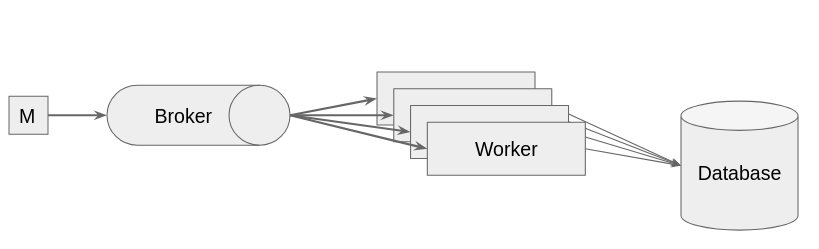
\includegraphics[width=0.8\textwidth]{fig/architecture.png}
  \caption{An architecture of a distributed task queue. Message \emph{M} is queued on the message broker, subsequently picked by workers which persist computed results into database.}
  \label{architecture}
\end{figure}

In many scenarios, having a single task for a request described by a message and processed by workers is not desired. In order to take advantage of horizontally scalable solution the request can be split into standalone units, called tasks, that compute one type of a result which can be additionally processed by other standalone tasks (also known as task flows, see below). The advantage of such logical split is mostly in possible paralelism and task retries in case of task failures. If a task fails, it can be retried without any negative impact on other independent tasks that can meanwhile run in parallel on different workers.

\section{Using Celery for Distributed Task Queue}

All of the objectives mentioned in the Section~\ref{section_distributed_task_queues} can be accomplished with stated open source solutions from Python ecosystem. In fact, we used Celery to accomplish desired behaviour. Celery offers "Celery primitives" that allow to model task flows\,--\,dependencies between tasks that can be eigher data dependencies (waiting for results of a task in order to start other tasks) or time dependencies (waiting on external events to proceed to next tasks). Celery primitives allow grouping tasks so tasks are executed in parallel or sequentially possibly on different workers in parallel.

An example of task flow modeling using Celery primitives can be seen on Figure~\ref{celery_phases} (the example is intentionally simplified, see Celery documentation~\cite{ref_celery_docs} for more in depth Celery primitives explanation). With Celery primitives we can create "phases" which group tasks that can be executed in parallel as there are no inter-task dependencies inside phases. Phases need to be executed one after another sequentially due to time or data dependencies of tasks that create these phases.

\begin{figure}
  \centering
  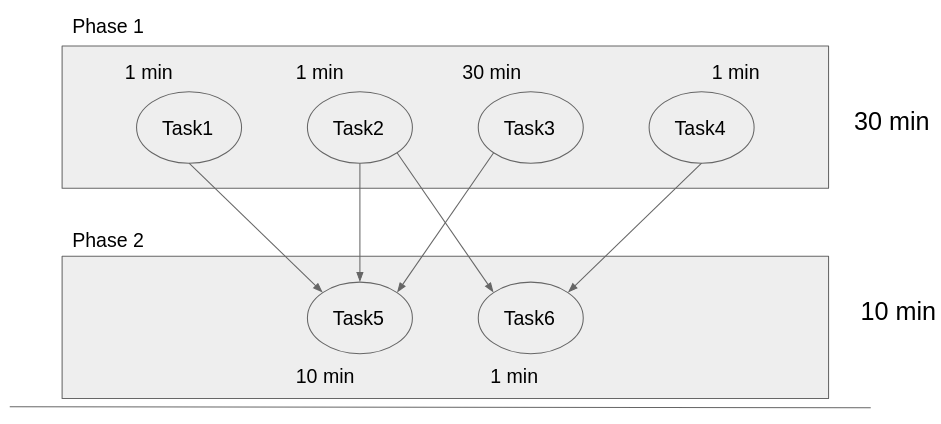
\includegraphics[width=0.8\textwidth]{fig/flow1.png}
  \caption{Phases created using Celery's primitives for tasks. Task \texttt{Task6} could be executed after 1 minute assuming \texttt{Task2} and \texttt{Task4} finish in one minute, but \texttt{Task3} blocks execution of \texttt{Task6}.}
  \label{celery_phases}
\end{figure}

The task flow made of phases using Celery's primitives is hard-coded inside application logic that makes application harder to maintain, harder to extend, more error prone with task or phase updates and adding a new task into an existing flow requires knowledge of internal dependencies of tasks that could be harder to see from source code. In the example above, the long running tasks block execution of tasks that could be already started respecting task flow dependencies.

\section{Orchestrating Task Flows with Selinon}

As we experienced drawbacks when using raw Celery, we managed to design a task flow orchestration tool on top of Celery which removes phase borders and all of the disadvantages stated above.

In the upcoming subsections, there are introduced Selinon abstractions. These abstractions create core components of Selinon design that act like a loosly coupled entities which, based on configuration, can create complex systems capable of serving large workload requests.

\subsection{Tasks and Task Flows}

A Selinon task is abstracted into a Python class respecting Selinon task interface. Implemented Selinon tasks are subsequently registered in the Selinon YAML~\cite{ref_yaml} configuration file and used to create task flows. The configuration of a flow states edges (or transitions) that model data or time dependencies between tasks. An example of such flow configuration can be seen on Figure~\ref{conf_flow}.

\begin{figure}[h!]
\begin{verbatim}
 flow-definitions:
   - name: flow1
       - from:
         to:
           - Task0
           - Task1
       - from: Task1
         to:
           - Task2
           - Task3
         condition:
           name: envExist
           args:
             name: PRODUCTION
\end{verbatim}
  \caption{An example of Selinon flow configuration.}
  \label{conf_flow}
\end{figure}

In the example shown in Figure~\ref{conf_flow}, Selinon starts \texttt{Task0} and \texttt{Task1}. Once \texttt{Task1} finishes, there are started tasks \texttt{Task2} and \texttt{Task3} that can run in parallel without possibly waiting for \texttt{Task0} to finish or fail. The \texttt{condition} section restricts \texttt{Task2} and \texttt{Task3} execution only for production systems (environment variable \texttt{PRODUCTION} is present). The conditional execution of tasks make the whole system dynamic\,--\,these conditions are evaluated each time an edge is fired and they can perform various actions such as checking external events or inspecting results of previous tasks. Their main purpose is to abstract away conditional task execution from actual task implementation logic as well as an optimization to prevent from queueing overhead needed to schedule unwanted tasks.

Besides scheduling tasks directly, Selinon is capable of creating nested flows\,--\,scheduling flows from within a flow. Moreover, the scheduling algorithm that Selinon offers removed a restriction on directed acyclic graph (DAG) in flow design which other open source alternatives have.

\subsection{Scheduling Algorithm}

The scheduling of tasks is done by a special message that is created per flow. This message keeps track of state in the flow. Each time a task or sub-flow is scheduled, the message carrying flow state information is updated and rescheduled with adjusted flow state. This mechanism allows to treat nested flows as any other task as the nested flow state is tracked in a separate newly created message referenced from the parent flow.

These special messages carrying flow state allow to sample state in the distributed environment as they are periodically scheduled and processed by wor\-kers.

\subsection{Storage and Database Adapters} \label{subsection_storage}

If there is a requirement for storing computed results there can be assigned storage adapters that handle task result storing and possible task result retrieval. In order to use an adapter, the adapter needs to be registered into the system in the YAML configuration file and assigned to a task.

This separation of task logic (how results are computed) from actual storing and retrieval mechanism allowed us to use transparently different storage and database solutions to store data in a way they could be later easily queryable based on data characteristics and query types we wanted to perform on computed results.

\subsection{Application Monitoring and Healthiness}

Selinon offers a built in support for application monitoring using flow tracepoints. Tracepoints are events that occur in cluster (such as a flow has started, a task has started, a task has failed) that help to monitor cluster behaviour. Selinon comes with a built-in support of error tracking software (such as Sentry~\cite{ref_sentry}) as well as structured well-defined logs that can be aggregated and further inspected using cluster-wide aggregated logging.

\section{Conclusion}


Selinon is an open source project, it's source code is available on GitHub~\cite{ref_selinon_github}. It is used in the OpenShift.io~\cite{ref_openshift_io} project for gathering and processing big data about packages in various ecosystems. With Selinon, we were able to create complex task flows that processed large amount of data stored in different database systems based on requirements. The configuration-centric design of loosely coupled components allowed us to perform system checks before actual deployment and gave us an ability to create easy to monitor dynamic system which behaviour can be changed even in online production systems without affecting already queued workload.

%
% ---- Bibliography ----
%
% BibTeX users should specify bibliography style 'splncs04'.
% References will then be sorted and formatted in the correct style.
%
% \bibliographystyle{splncs04}
% \bibliography{mybibliography}
%
\begin{thebibliography}{8}
\bibitem{ref_selinon_homepage}
Selinon project homepage, \url{https://selinon.readthedocs.io/}. Last accessed 28 May 2018

\bibitem{ref_selinon_github}
Selinon project on GitHub, \url{https://github.com/selinon/}. Last accessed 28 May 2018

\bibitem{ref_celery}
Celery project homepage, \url{https://celeryproject.org}. Last accessed 28 May 2018

\bibitem{ref_celery_docs}
Celery project documentation, \url{docs.celeryproject.org/}. Last accessed 28 May 2018

\bibitem{ref_yaml}
The Official YAML Web Site, \url{http://yaml.org/}. Last accessed 28 May 2018

\bibitem{ref_openshift_io}
OpenShift.io: An Open Online Development Environment, \\ \url{https://www.openshift.io}. Last accessed 28 May 2018

\bibitem{ref_airflow}
Apache Airflow documentation, \url{https://airflow.apache.org}. Last accessed 28 May 2018

\bibitem{ref_luigi}
Spotify Luigi project on GitHub, \url{https://github.com/spotify/luigi}. Last accessed 28 May 2018

\bibitem{ref_sentry}
Sentry: Error Tracking Software, \url{https://sentry.io}. Last accessed 28 May 2018
\end{thebibliography}

%=============================================================================

%\bigskip
%\noindent \textbf{Poděkování:} Tento článek vznikl díky částečné podpoře projektů \dots

\end{document}
